\section{Behavioral Attestation for AI Agents}
\label{aegis}

We propose behavioral attestation as the foundation for securing AI agents in HPC. We implement this concept in \projectname~(Attestation-based Environment for Guarding Injection-vulnerable Systems).

\subsection{Overview}

\begin{figure*}[!t]
  \centering
  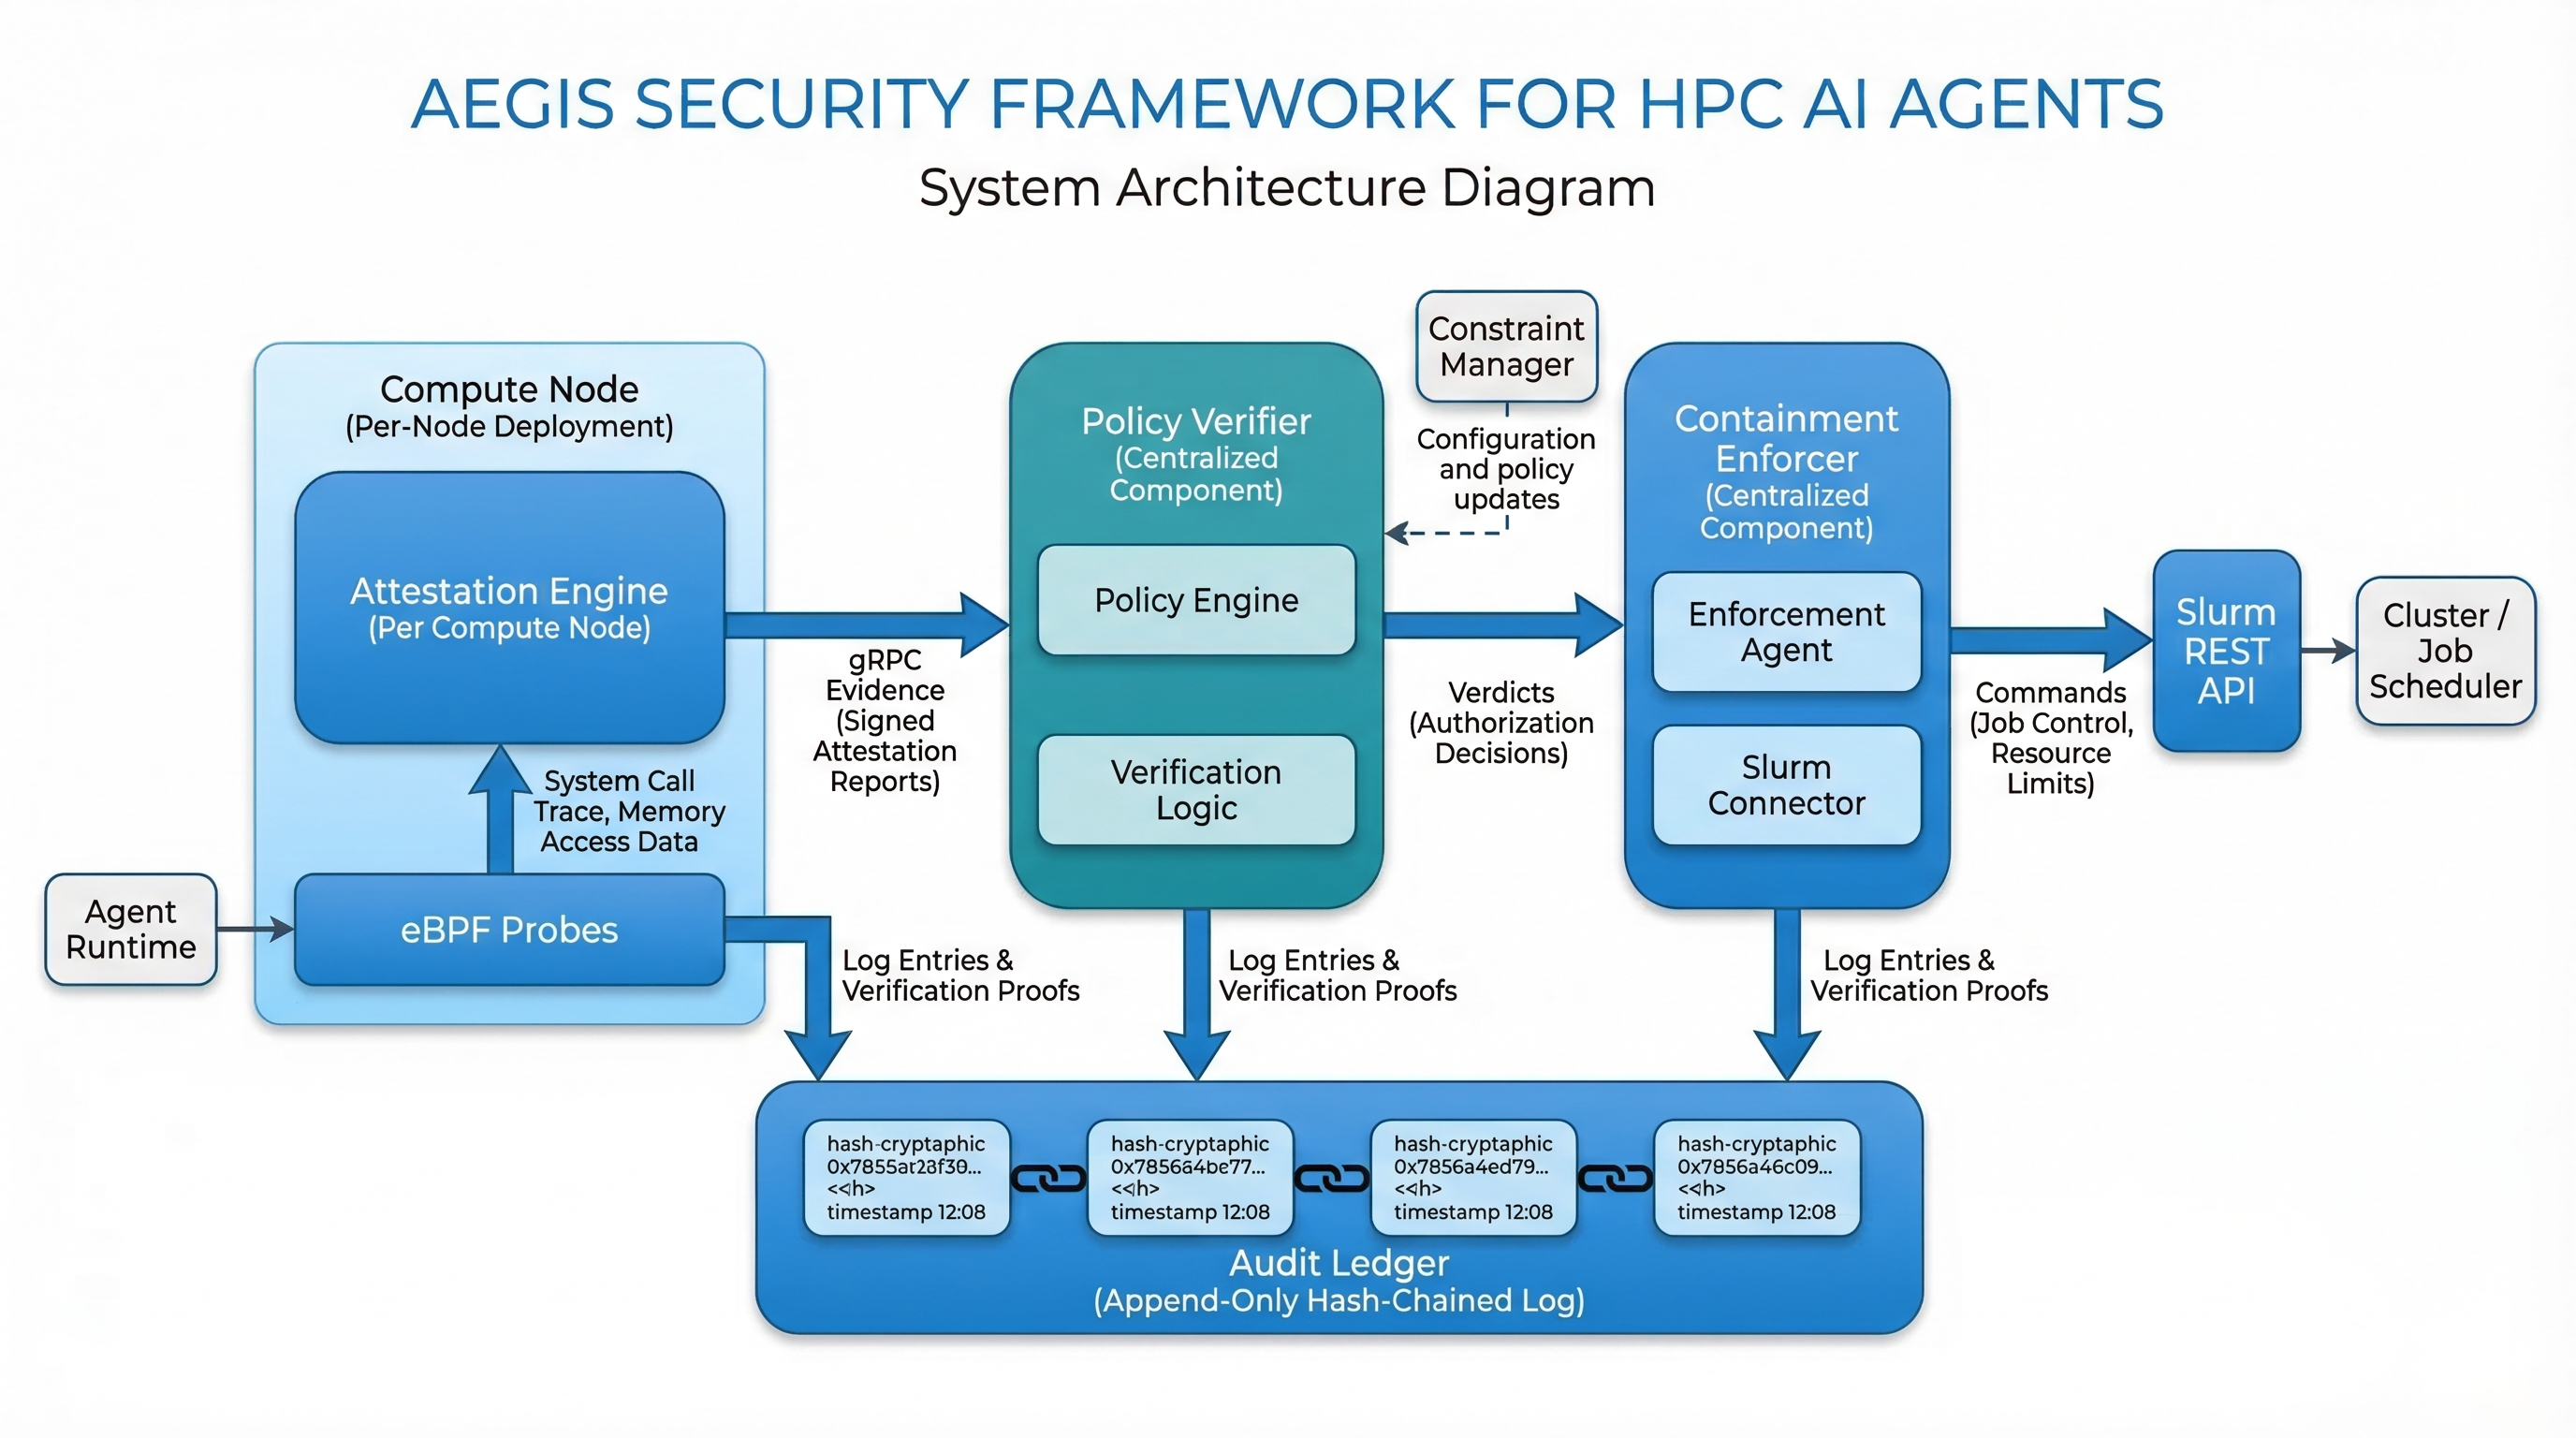
\includegraphics[width=0.70\linewidth]{../figures/aegis_architecture.png}
  \caption{Overview of the \projectname~system architecture. Four core components: Attestation Engine (per-node, \ebpf-based), Policy Verifier (centralized), Containment Enforcer (Slurm REST API), and Constraint Manager. }
  \label{fig:aegis_arch}
\end{figure*}

Figure~\ref{fig:aegis_arch} illustrates the \textit{four} core components of \projectname~that operate across the HPC cluster. The \textit{Constraint Manager} parses and compiles behavioral constraint profiles into an internal policy representation. It supports explicit specification, task inference, and policy templates. Profiles are signed and bound to the agent's Slurm job ID. The \textit{Attestation Engine} runs as a daemon on each compute node, intercepting agent system calls via \ebpf probes. It produces signed attestation evidence bundles at configurable intervals, transmitted to the verifier over mutually authenticated gRPC. The \textit{Policy Verifier} is a centralized service that evaluates evidence against constraint profiles, producing verdicts ranging from \texttt{COMPLIANT} to \texttt{VIOLATION-CRITICAL}. It issues random challenges to prevent delayed reporting and maintains a shared access graph across all attested agents on the cluster, enabling cross-agent correlation to detect coordinated attacks such as covert channels via shared filesystem paths. The verifier correlates write-read patterns across agent sessions: if Agent A writes to a path and Agent B reads from the same path within a sliding time window, this triggers a covert channel alert. All decisions are logged to a tamper-evident audit ledger. The \textit{Containment Enforcer} translates verdicts into enforcement actions via the Slurm REST API. It supports cgroup throttling for minor violations, ACL revocation for moderate violations, job suspension for severe violations, and termination with credential revocation for critical violations.

These components implement behavioral attestation, a fundamentally new concept that differs from prior approaches along \textit{three} axes. Prior approaches provide detection through probabilistic mechanisms such as ML-based classifiers with inherent false positive and negative rates. Behavioral attestation provides deterministic constraint verification with optional signature augmentation. Prior approaches use signature-based policies that block known-bad patterns which can be evaded through obfuscation. Behavioral attestation uses constraint-based policies that define what is allowed, where violations are unambiguous. Prior approaches operate post-hoc, alerting after the attack succeeds when damage is already done. Behavioral attestation operates at runtime, detecting and containing violations during execution.

The key insight underlying our approach is that we cannot prevent all injection attacks because the attack surface is too large and too diverse. However, we can \textbf{detect and contain the effects of hijacked agents by attesting to behavioral constraints}. \projectname~uses a hybrid detection model: constraint-based verification serves as the primary mechanism and ensures that agent actions conform to declared behavioral boundaries. An optional signature layer augments detection with known injection patterns for specific attack vectors. The constraint layer alone achieves 75\% detection as shown in the ablation study, and signatures boost this to 100\% for attacks that produce recognizable patterns.

\subsection{Behavioral Constraint Profiles}

Each agent receives a behavioral constraint profile at deployment, declarations of legitimate behavior derived from the agent's authorized task, not signatures of malicious behavior. Constraints span five dimensions: \textit{data access} (allowed/denied paths, read-only paths, volume limits), \textit{network} (whitelisted endpoints, egress budgets), \textit{tool invocation} (allowed/denied tools), \textit{execution} (runtime limits, memory limits, node restrictions), and \textit{data flow} (project boundaries, cross-agent isolation). Constraints are evasion-resistant: an attacker cannot make an unauthorized action authorized through obfuscation; the constraint either permits the action or it does not. Cross-agent constraints specify whether the agent may share data with other agents, access co-located agent outputs, or participate in inter-agent communication channels.

We support three modes of constraint derivation. Explicit specification allows users to declare constraints directly through a declarative YAML-based language. Task inference uses an LLM to analyze the agent's task description and automatically generate appropriate constraints. Policy templates provide pre-built constraint sets for common HPC agent patterns such as data analysis, simulation steering, and ML training.

The constraint profile is cryptographically bound to the agent's execution context. We link the profile to the agent's Slurm job ID, creating a verifiable binding between the authorized behavior and the running process. This prevents an attacker from substituting a more permissive profile.

\subsection{Attestation Evidence}

The Attestation Engine monitors agent behavior through \ebpf-based syscall interception~\cite{gregg2020bpf}. The engine hooks six syscall tracepoints: \texttt{sys\_enter\_openat} for file access detection, \texttt{sys\_enter\_read} and \texttt{sys\_enter\_write} for byte counters, \texttt{sys\_enter\_connect} for network connections, \texttt{sys\_enter\_sendto} for network egress tracking, and \texttt{sys\_enter\_execve} for tool invocations. Events are emitted via the BPF ring buffer to userspace, and Section~\ref{results} quantifies both worst-case syscall overhead and end-to-end verifier cost on the deployed path. The probe tracks per-PID state including cumulative bytes read and written, and connection counts.

At configurable intervals (default: 1 second), the Attestation Engine produces a signed attestation evidence bundle containing the agent's access log, data volume counters, hash of the agent's process state, and a cryptographic signature. The evidence bundle is transmitted to the Policy Verifier for evaluation.

\subsection{Policy Verification}

The Policy Verifier evaluates evidence bundles against constraint profiles, producing verdicts that indicate the severity of any violations. The verdict scale ranges from \texttt{COMPLIANT} (no violations) through \texttt{VIOLATION\_MINOR}, \texttt{VIOLATION\_MODERATE}, \texttt{VIOLATION\_SEVERE}, to \texttt{VIOLATION\_CRITICAL} (severe threat requiring immediate action).

The verifier maintains a cluster-wide access graph that tracks all agent filesystem and network interactions across all compute nodes. This enables cross-agent correlation to detect coordinated attacks. The verifier correlates write-read patterns across agent sessions: if Agent A writes to a path and Agent B reads from the same path within a sliding time window, this triggers a covert channel alert. The time window and correlation thresholds are configurable.
% To prevent delayed reporting attacks, the verifier issues random challenges at Poisson-distributed intervals, requesting on-demand attestation from a randomly selected agent. This ensures that agents cannot predict when they will be audited and therefore cannot selectively report compliant behavior.
All verification decisions are logged to a tamper-evident audit ledger. The ledger uses a cryptographic hash chain, enabling post-hoc forensic analysis and detection of log tampering.

\subsection{Containment Enforcement}

The Containment Enforcer translates verification verdicts into enforcement actions through the Slurm REST API. Four escalation levels are supported. For minor violations, the enforcer applies cgroup-based rate limiting, throttling the agent's CPU and memory resources. For moderate violations, the enforcer revokes filesystem ACLs, isolating the agent from shared storage. For severe violations, the enforcer suspends the Slurm job, pausing agent execution. For critical violations, the enforcer terminates the job and revokes credentials, ensuring the compromised session cannot be reused.

% We measure the time from violation detection to enforcement action. At a 1-second attestation interval, the maximum detection latency is 1 second plus evaluation time, which we measure at less than 0.5ms. Combined with Slurm API latency, total containment time is under 2 seconds.

\subsection{Optional Signature Layer}

For deployments requiring maximum detection coverage, \projectname~includes an optional signature-based augmentation layer. This layer detects known prompt injection patterns in tool outputs and inter-agent messages using pattern matching against a curated database of injection signatures such as hidden instruction patterns and base64-encoded commands. The signature layer is disabled by default and must be explicitly enabled; it is not required for constraint-based detection to function. In the controlled synthetic ablation, the non-signature mechanisms detect 3 of 4 attacks (75\%), and enabling injection signatures raises detection to 4 of 4 by catching the crafted supply-chain attack.

\subsection{Implementation Details}

\projectname~is fully implemented as a modular system. The implementation consists of approximately 4,500 lines of code. The C \ebpf probe provides kernel-side syscall hooks, and the Python collector reads from the ring buffer to assemble evidence bundles. The centralized verifier maintains the cluster-wide access graph and tamper-evident audit ledger, while the evaluation harness instantiates the baseline DLP, auditing, analytics, and sandbox comparators used in Section~\ref{results}. The \slurm{} integration layer translates verifier decisions into containment actions through the REST API. The implementation is released with the artifact for reproducibility.

